\documentclass{article}
\usepackage{graphicx}
\usepackage{geometry}
\usepackage[fleqn]{amsmath}
\usepackage{tikz}
\usepackage{hyperref}
\newgeometry{left=3cm, top=2cm, bottom=2cm}
\graphicspath{{./img/}}
 	
%Path in Unix-like (Linux, OsX) format
\begin{document} 
	\title{Artificial Neural Networks - Torch + Lua}
	\author{Arulkumar S (CS15S023)}
	\maketitle 

	\section{Introduction to Torch}
	
	\subsection{Setup}
	The startup code\cite{stmt} is downloaded and the main file (qlua
	\href{./SVHN_training/1_data_SVHN_dataset.lua}{1\_data\_SVHN\_dataset.lua}) is
	executed in the PC to train the already defined model upto 15 epochs. \\\\
	The required SVHN dataset\cite{svhn}, MNIST dataset\cite{mnist} are
	downloaded from it's source websites.\\\\ The time taken to complete one epoch with full dataset (73257
	examples) = approx. 45 minutes \\\\
    The time taken to complete one epoch with reduced (small) dataset(10000
	examples) = approx. 10 minutes
	
	\subsection{Testing and Visualization}
	
	The trained model (with SVHN dataset upto ~15 epochs) is
	\href{./testing_visualization/testTheModel.lua}{loaded independently} \& tested
	with one of the images of numbers. \\\\ The convolution layer outputs are shown
	below:\\\\
    \textbf{Test image}\\\\
    \includegraphics[scale=1]{originaltestimg}\\\\
	\textbf{Snapshot of filtered images from 1st convolution layer}\\
	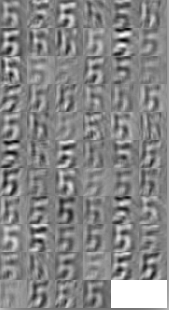
\includegraphics[scale=0.4]{1stfilterLayer}\\\\
    \textbf{Snapshot of filtered images from 2nd convolution layer}\\
    \includegraphics[scale=0.6]{2ndfilterLayer}
       
    \newpage
	\subsection{Transferring the knowledge}
	
	The saved model (trained in SVHN dataset) can then be loaded independently of
	the training/test data \& can be used to predict the numbers in image.\\\\
	Since, the previous SVHN model is trained using RGB images, we will not be able
	to use the model for MNIST dataset, as MNIST contains images are of only Gray color.
	\\\\So, as a first step, all the images in SVHN training dataset are converted
	to Gray image and used to train the model again.\\\\I observed that there is a
	minor deviation between the notation of labels used in SVHN \& MNIST datasets.
	The label settings in these two datasets are as below:
	
	\begin{center}
	  \begin{tabular}{ c | c | r | l }
		\multicolumn{1}{c}{Number in the image} & 
		\multicolumn{1}{c}{SVHN label} & 
		\multicolumn{1}{c}{MNIST label}\\
	    \hline
	    0  & 10& 1 \\
	    1  & 1 & 2 \\
	    2  & 2 & 3 \\
	    3  & 3 & 4 \\
	    4  & 4 & 5 \\
	    5  & 5 & 6 \\
	    6  & 6 & 7 \\
	    7  & 7 & 8 \\ 
	    8  & 8 & 9 \\ 
	    9  & 9 & 10 \\
	    \hline
	  \end{tabular}
	\end{center}
	To equalize the labels between SVHN \& MNIST datasets, the labels in MNIST
	datasets are subtracted by 1 \& if the label is 0, then it is filled by
	10.\\\\Now, As per the requirement, the model is trained with SVHN dataset (for
	10 epochs)) and tested with MNIST test dataset.\\\\The observations are:
	\begin{list}{*}{}
	  \item Even after 10 epochs, the MNIST test set accuracy (68.1\%) is less
	  compared to the SVHN training set accuracy (96.375\%)
	  \item Though the SVHN training dataset error reduces fast during training,
	  the MNIST test set performance is not good
	\end{list}
	The detailed log can be found
	\href{./MNIST_test_with_SVHNmodel/results/SVHN_MNIST_trace.log}{here}.\\\\
	After getting a trained model from SVHN dataset, the same trained model is
	provided with the training data from MNIST dataset and trained for
	about 10 epochs.\\\\The observations are:
	\begin{list}{*}{}
	  \item In the $1^{st}$ epoch, The test set accuracy is dramatically increased
	  to 96\% due to parameter fine-tuning.
	  \item At the end of $3^{rd}$ epoch, the training set accuracy is reached
	  99.2\%
	\end{list}
	The detailed log can be found
	\href{./MNIST_test_with_SVHNmodel/results/SVHN_MNIST_trace.log}{here}.\\\\
	\newpage
	\textbf{during epoch\#10 with SVHN training dataset \& MNIST test dataset}\\\\
	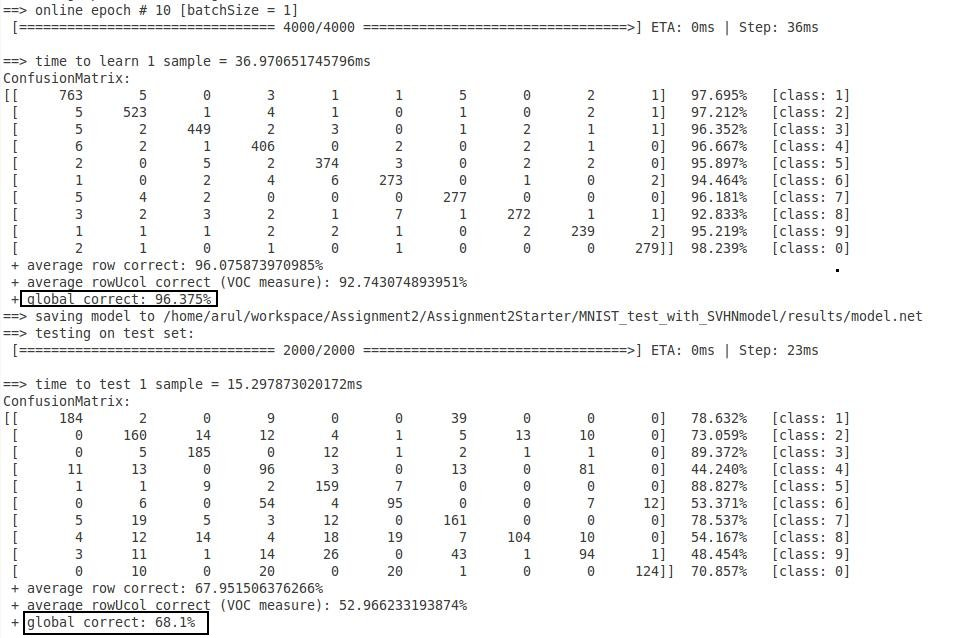
\includegraphics[scale=0.4]{./MNIST_test_with_SVHNmodel/results/svhn+mnist.jpg}\\\\
	\textbf{during epoch\#10 with MNIST training dataset \& MNIST test dataset}\\\\
	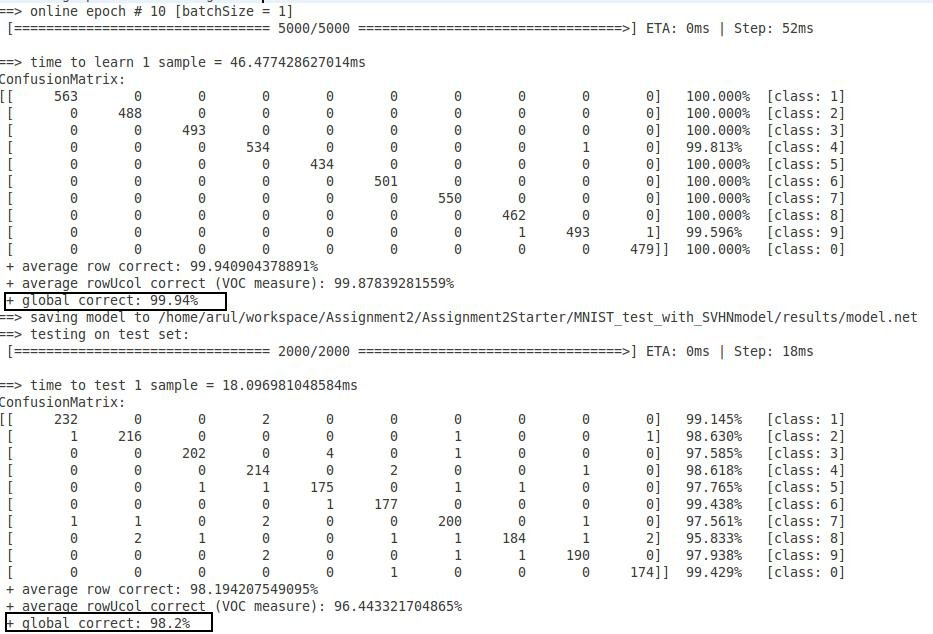
\includegraphics[scale=0.4]{./MNIST_test_with_SVHNmodel/results/mnist+mnist.jpg}
	\newpage
	\section{Own layer in Neural network}
	
	\subsection{'ReQU' unit}
	\href{./ReQUlayer/requ.lua}{source code}
	\\\\
	As per the given definition of $ReQU$ unit, the implementation is done in
	$updateOutput()$ \& $updateGradInput()$ function.\\\\
	ReQU function output\\\\
	\begin{equation*}
	 z_{i} =  \begin{cases} 
					0, & x_{i}\leq 0 \\
					x^{2}, & x > 0 \\
			  \end{cases}
	\end{equation*}
	\\\\
	The unit testing of the new ReQU layer is done
	using the \href{./ReQUlayer/requTest.lua}{unit test file}. To test the
	model of ReQU, a new object of ReQU is created \& the data is passed to the
	function $model:forward()$ \& the output is verified.\\\\
	The test log can be found
	\href{./ReQUlayer/requTest.log}{here}.
	\subsection{Testing the module on full network}
	The simple network used for testing ReQU is having the layered form as:
	\begin{verbatim*}
linear->ReQU->linear->softmax
	\end{verbatim*}
	~\newline For testing the gradient calculation done on the ReQU function
	$updateGradInput()$, an approximation method as shown below, is followed to
	estimate the expected Gradient.
	\begin{equation*} 
	\frac{\partial E}{\partial w_{i}} = \frac{f(w_{1}, w_{2}, \ldots, w_{i} +
	\epsilon, \ldots, w_{n}) - f(w_{1}, w_{2}, \ldots, w_{i} - \epsilon, \ldots,
	w_{n})}{(2*\epsilon)}
	\end{equation*}
	\\\\The $\epsilon$ is chosen as $10^{-7}$.\\\\The
	measure of Symmetric relative error\cite{stmt}\cite{oxford} is found between the Actual gradient ($g1$) \&
	Estimated gradient ($g2$) as,\\\\Relative error = $\frac{||g1 - g2||}{2 *||g1 +
	g2||}$\\\\It is observed that the symmetric
	relative error is close to the chosen $\epsilon$.\\\\Also, the cosine
	similarity measure is calculated as, \\\\ cosine-similarity(actualGradient($g1$), estimatedGradient($g2$)) = $\frac{g1^{T}g2}{|g1|.|g2|}$ \\\\The calculated
	cosine similarity is very close to 1. \\\\Hence, the results show that the
	$updateGradInput()$ function in new module 'ReQU' is performing as expected. \\\\
	The measures taken can be seen in the
	\href{./ReQUlayer/gradientsTest.txt}{Log file}
		
	\bibliographystyle{plain}
	\bibliography{mybib}
	
	
\end{document}